\def\topfraction{.9}
\def\floatpagefraction{.8}

%=========================================================================
\chapter{Úvod}
V~moderních operačních systémech určených pro desktop (pracovní stanice,
notebooky, etc.) se oproti předchozím verzím změnilo mnohé. Jednou takovou
změnou je~změna bezpečnostní politiky.

MS Windows postupně získal mnohem lepší zabezpečení ve verzích NT, kdy došlo
k přechodu na nové jádro, a Vista, kde se poprvé objevila možnost jednoduše
povolit obyčejnému uživateli přístup k nastavení systému pomocí UAC>citace<.
Zamezilo se tak nutnosti 'být administrátorem', což bylo do té doby výchozí
nastavení po intalaci. Ve výsledku má uživatel povoleny akce, ke kterým by jinak
přístup neměl.

Unixové a unixu podobné systémy se vyvíjely směrem opačným -- od práv pevně
svázaných s jeho účtem a skupinou, k mnohem volnějšímu pojetí. V oblasti unixu
a unixu podobných systémů za zmínku stojí například program sudo
[ref:http://www.sudo.ws/sudo/history.html], který umožňuje uživateli spouštět
programy s jinými právy než jsou jeho vlastní (převážně superuživatelská práva)
případně program su, který je ještě staršího data.

Nově je k dispozici také PolicyKit >citace<, který plní podobnou úlohu jako UAC
na OS Windows. Aplikace využívající PolicyKit nemusejí mít pro změnu systémového
nastavení jako je třeba datum a čas superuživatelská práva.

Prostředí KDE >citace< (po přeznačení KDE Software Compilation) je možné
provozovat na více operačních systémech. Aplikace by tak musely používat řešení
jako je UAC nebo PolicyKit, což by omezilo jejich přenositelnost. Tyto řešení
tedy bylo potřeba nějak obalit. Za tímto účelem vzniklo rozhraní KAuth>citace<.

V rámci KDE však bylo možné již dřive měnit práva uživatelů - skrývat položky
menu, zamezit použití terminálu a podobně. K tomu slouží Kiosk>citace<
-- kombinace vlastností několika systémů obsažených v KDE.

Tyto technologie a způsob jakým budou v práci využity jsou blíže popsány ve
druhé kapitole>ref<.

Cílem této práce je:
\begin{itemize}
\item Změnit API KAuthorized tak, aby používalo KAuth pro akce a zdroje (Actions
 and Resources) - viz. kapitola 3
\item Převést nástroj KioskTool do prostředí KDE4 -- kapitola 4
\item Vytvořit nástroj pro migraci nastavení ze systému KConfig do nového KAuth
-- kapitola 5
\item A na závěr ověřit funkčnost řešení a připravit jej na začlenění do KDE
knihoven (KDELibs)
\end{itemize}

\chapter{Základní technologie}
V této kapitole popíši blíže zmíněné rozhraní a aplikace, tak aby bylo jasné jak fungují
a jaké podmínky musí být splněny, aby bylo výsledné řešení ekvivalentem původního.

Dříve než se pustíme do samotného popisu technologií je třeba vymezit některé pojmy:
KAuth -- rozhraní nad autorizačním řešením jako je například PolicyKit.

KConfig -- Systém pro ukládání a načítání nastavení v KDE.

Kiosk -- Souhrnný pojem pro některé vlastnosti KConfigu.

Kiosk profil -- Profil přiřazený uživateli nebo skupině uživatelů, má vyšší prioritu
než normální uživatelská nastavení KDE, ale nižší než globální systémové nastavení.

KAuthorized -- tenké rozhraní nad KConfigem/Kioskem, umožňující dotazování, zda
jsou některé typy akcí povoleny.

KioskTool -- aplikace pro správu tzv. Kiosk profilů. V KDE 3 umožňovala jednoduše
nastavit některé části systému Kiosk/KConfig bez nutnosti měnit Kiosk profily ručně.

\section{Kiosk}
%ref: http://techbase.kde.org/KDE_System_Administration/Kiosk/Introduction
Z pohedu administrátora Kiosk nabízí možnost upravit si KDE pro své vlastní
účely. Například schovat některé položky v grafickém rozhraní aplikací,
znemožnit uživatelům měnit nastavení a data aplikací nebo zamezit spuštění
terminálu. Toho je docíleno nastevením některých částí konfigurace jako
nezměnitelné (immutable) nebo vytvořením tzv. Kiosk profilů a přiřazením těchto
profilů k uživatelům a skupinám. Tyto profily jsou složky obsahující v zásadě
stejné soubory jako používá KConfig.

Kiosk je obecný pojem pro několik rozdílných vlastností systému KConfig a s ním
provázanými částmi KDE. Nelze přesně určit jedno konkrétní místo ve zdrojovém kódu
KDE, kde by bylo popsáno jakým způsobem funguje, ale podrobným zkoumáním lze vysledovat,
jak je docíleno výsledného efektu. Z velké části je funkce Kiosku závislá na funkci
KConfigu a způsobu jakým jsou načitány Kiosk profily během spouštění KDE aplikací
a jejich komponent. Toto si blíže popíšeme, protože je to podstatné pro pochopení
řešeného problému.

\subsection{Načítání konfigurace během spuštění aplikace}
Každá KDE aplikace má několik základních částí, obsažených ve struktuře KGlobal.

            ::obrázek
            KGlobal --|-- KComponentData --|-- KAboutData
                      |                    |-- KStandardDirs
                      |                    |-- KSharedConfig
                      |-- Locale
                      |-- nadpis okna

KGlobal je jmenný prostor obalující přístup k dalším komponentám a sdíleným
zdrojům v rámci aplikace.
KComponentData obsahuje informace relevantní pro jednu komponentu aplikace.
Platí, že aplikace může mít jednu hlavní komponentu.
KAboutData obsahuje základní informace o programu komponentě -- v případě hlavní
komponenty jsou tyto informace použity také pro dialog 'O Aplikaci' (About).
Je nutno poznamenat, že aplikace může mít více než jednu komponentu.
KSharedConfig zajišťuje, že konfigurace je sdílena mezi komponentami -- šetří
se tak pamětí a CPU časem nutným k načtení konfigurace.

KStandardDirs slouží k určení, které složeky budou použity jako zdroj dat
a konfigurace pro aplikaci.
KSharedConfig obsahuje sloučenou konfiguraci, efektivní pro program.

Právě KStandardDirs a KSharedConfig jsou relevantní pro popis načítání
konfigurace. Během inicializace komponenty se nejdříve načítá obecná konfigurace
>ref void KComponentDataPrivate::lazyInit<. Ta obsahuje nastavení pro celé KDE
a zmíněnou aplikaci, ovšem bez začleněných Kiosk profilů. Tato kofigurace
obsahuje také odkazy na Kiosk profily pro jednotlivé uživatele a skupiny. Jak
již bylo řečeno, Kiosk profily jsou složky se stejnými konfiguračními soubory
jako používá KConfig.

Potom je volána metoda KStandardDirs::addCustomized, která vyhledá Kiosk profily
platné pro uživatele (na *nix systémech je soubor s jejich seznamem odkazován z
'/etc/kderc') a zařadí je s prioritou (narozdíl od cest ke zdrojům určených
v konstruktoru KStandarDirs jsou umístěny na začátek seznamu složek
s konfiguračními zdroji).

Platí, že pokud má uživatel přiřazen svůj vlastní Kiosk profil, nezpracovávají
se dále Kiosk profily pro skupiny v nichž je členem. V opačném případě, kdy
uživatel nemá vlastní profil, přidají se s prioritou do cest v KStandardDirs
všechny aplikovatelné skupinové profily. Pokud se počet cest s konfigurací
změnil, je po návratu z addCustomized konfigurace znovu načtena.

\subsection{KConfig}
Kconfig je, jak již bylo řečeno, systém pro načítání a ukládání nastavení v KDE.
V základu je navržen tak, aby bylo možné použít různé způsoby uložení nastavení,
ale v praxi jsou použity .ini soubory (jsou jednoduché a rychle se načítají).

Ukázka souboru '/etc/kde4rc':
\begin{verbatim}
[Directories]
kioskAdmin=kde-devel:
userProfileMapFile=/etc/kde-user-profile

[Directories-default]
prefixes=/etc/kde-profile/default/

[Directories-profile1]
prefixes=/etc/kde-profile/profile1/

[Directories-test]
prefixes=/etc/kde-profile/test/

[Directories-testprof]
prefixes=/etc/kde-profile/profile2/
\end{verbatim}
Zde je vidět, jak je soubor členěn. Obsahuje skupiny a záznamy typu
klíč-hodnota. Soubory se během načítání konfigurace slučují do jednoho
konfiguračního celku
(třída KConfig).

\subsubsection{Nezměnitelnost (Immutability)}
Celé soubory, skupiny jako je 'Directories' a jednotlivé záznamy jako je např.
'prefixes' je možné nastavit jako nezměnitelné -- 'immutable' pomocí přidání
značky [\$i].
Jakmile je jednou nastavena na skupinu, soubor nebo hodnotu nezměnitelnost, jsou
další objekty stejného typu při načítání ignorovány. Máme-li tedy pro uživatele
'test' nastaven Kiosk profil 'testprofil', který obsahuje například konfigurační
soubor pro aplikaci Akragator, nastavený jako nezměnitelný, nebude moci uživatel
nastavení tohoto programu změnit.

\subsection{KAuthorized}
Toto rozhraní (přesněji jmenný prostor) je tenkým obalem nad KConfigem, který
využívá všech jeho vlastností. Poskytuje KDE knihovnám a aplikacím možnost
autorizace obecných akcí, KAkcí (KAction), konfiguračních modulů KCM, a přistupů
k URL adresám.
Chybí zde ovšem omezení přístupu ke zdrojům.

\subsubsection{KAkce (KActions) a obecné akce}
Nastavované ve skupině 'KDE Action Restrictions'.
Rozdíl mezi obecnou akcí a KAkcí v rámci KAuthorized je mizivý a funkce
AuthorizeKAction je obal nad authorize(), který před název akce přidá prefix
'action/'.

V rámci KDE jsou akce (třída KAction odvozená od QAction z knihovny QT) obecně
činnosti, které může uživatel vykonat v rámci aplikace. Tyto akce mají název,
který je v Kiosku použit pro jejich autorizaci. Funkce AuthorizeKAction tedy
dostane od aplikace název akce, přidá před něj již zmíněný prefix a pokusí se
o autorizaci pomocí KConfigu.
Akce může být například otevření menu s nápovědou. Pokud je taková akce zakázána
pomocí Kiosku, menu se nezobrazí.

\subsubsection{Omezení přístupu ke zdrojům}
Nastavované ve skupině 'KDE Resource Restrictions' a umístěné do globálního
konfiguračního souboru jako je 'kdeglobals'.
I když je tato část Kiosku velmi podobná ostatním autorizačním funkcím
v KAuthorized, není do něj přímo začleněna.

Důvodem je, že je úzce provázána s třídou KStandardDirs, která tyto omezení
zpracovává a používá pro vytvoření seznamů složek se zdroji. Seznam těchto
omezení je totiž potřeba znát ještě před tím, než je zcela načtena konfigurace.
To by však nemělo bránit vytvoření nové funkce pro získání seznamu typu zdrojů
s omezením přístupu v jmenném prostoru KAuthorized (mohla by například vracet
QStringList).

\subsubsection{Omezení přístupu k URL}
%ref: http://techbase.kde.org/KDE_System_Administration/Kiosk/Introduction#KDE_URL_Restrictions
Nastavované ve skupině 'KDE URL Restrictions', tyto omezení jsou určeny
pro zamítnutí přístupu k některým adresám URL. Vstupní parametry jsou seznam
šestic hodnot a ověřovaná URL.

Syntaxe pro takovouto šestici:
\begin{verbatim}
rule_N=<action>,<referrer protocol>,<referrer host>,<referrer path>,
    <protocol>,<host>,<path>,<enabled>
\end{verbatim}

Jednotlivé části je možné vynechat nebo místo nich použít proměnné jako
je \$HOME nebo \$TMP.

Příklad:
\begin{verbatim}
[KDE URL Restrictions][\$i]
rule_count=6
rule_1=open,,,,file,,,false
rule_2=list,,,,file,,,false
rule_3=open,,,,file,,\$HOME,true
rule_4=list,,,,file,,\$HOME,true
rule_5=open,,,,file,,\$TMP,true
rule_6=list,,,,file,,\$TMP,true
\end{verbatim}

Pravidla 1 a 2 jsou vypnuta, 3 - 6 zakazují otvírat a vypisovat soubory
v \$HOME a \$TMP.

\subsubsection{Omezení přístupu ke KCM modulům}
Kde používá třídu KCModule jako základ pro všechny moduly použité v aplikacích
'Nastavení Systému' a kcmshell. Za pomoci těchto omezení je možné skrýt
tyto moduly ve zmíněných aplikacích a tam kde je možné je jinak otevřít tak,
aby je uživatel nemohl otevřít. To stejné funguje i pro služby KDE (KService).

\subsection{KioskTool}
Aplikace KioskTool umožňovala v KDE 3 spravovat některé specifické části Kiosk
profilů pomocí grafického rozhraní. Najprve popíši její funkčnost ve verzi pro
KDE3 za pomocí obrázků, protože tak to bude nejlepší. Také se zmíním
o nedokončeném pokusu o převedení této aplikace do KDE4 a nedostatcích v obou
verzích.

\begin{figure}[h]
    \centering
    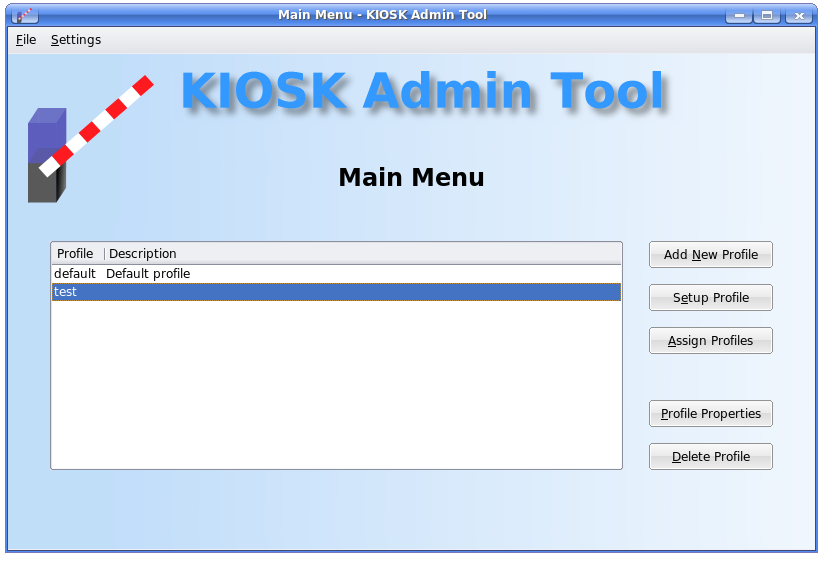
\includegraphics[width=8.5cm]{obrazky/KioskToolKDE3/uvodni_obrazovka.png}
    \caption{Úvodní obrazovka programu}
    \label{fig:kt3_uvodni}
\end{figure}
Úvodní obrazovka \ref{fig:kt3_uvodni} ukazuje seznam profilů s jejich popisem,
lištu s menu a tlačítka pro manipulaci s profily. Velmi chybí možnost zkopírovat
již existující profil.

\begin{figure}[h]
    \centering
    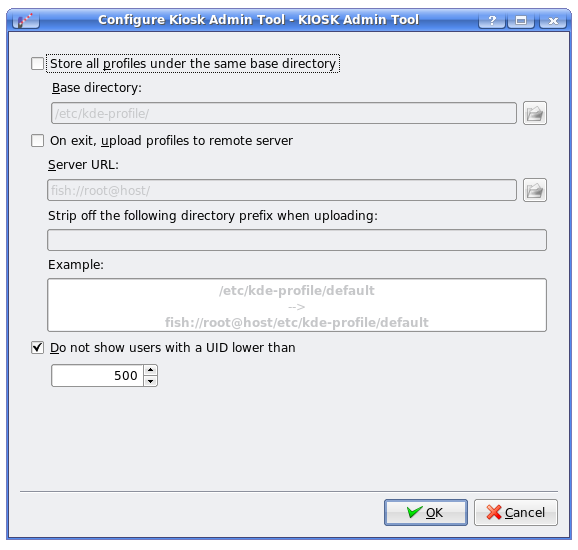
\includegraphics[width=8.5cm]{obrazky/KioskToolKDE3/nastaveni.png}
    \caption{Dialogové okno s nastavením}
    \label{fig:kt3_nastaveni}
\end{figure}
Mezi nastavení programu \ref{fig:kt3_nastaveni} patří také možnost automaticky
uložit profily na vzdálený serber.

\begin{figure}[h]
    \centering
    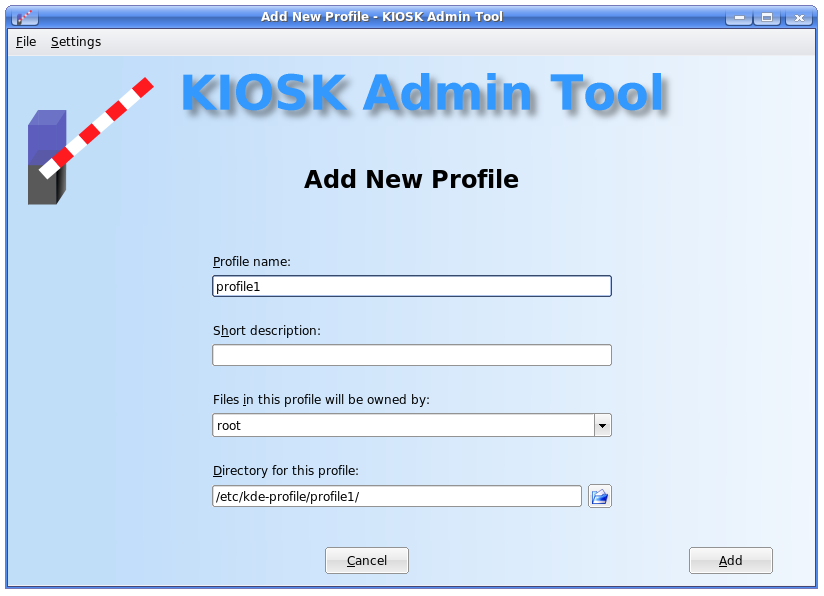
\includegraphics[width=8.5cm]{obrazky/KioskToolKDE3/novy_profil.png}
    \caption{Dialog pro vytvoření nového profilu}
    \label{fig:kt3_novyprofil}
\end{figure}
Dialog pro vytvoření nového profilu \ref{fig:kt3_novyprofil} je poměrně
jednoduchý. Umožňuje nastavit název a popis profilu a dále který uživatel bude
vlastnit složku s profilem (bude mít přístup pro zápis) a kde bude profil
uložen.

\begin{figure}[h]
    \centering
    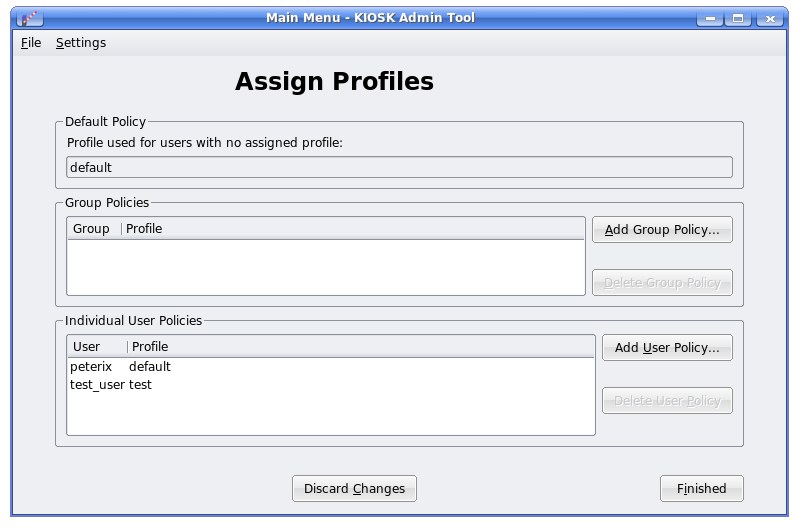
\includegraphics[width=8.5cm]{obrazky/KioskToolKDE3/prirazeni_profilu.png}
    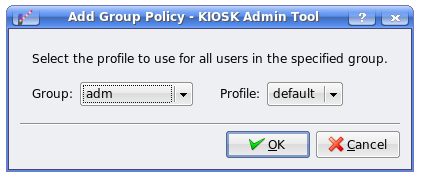
\includegraphics[width=8.5cm]{obrazky/KioskToolKDE3/prirazeni_profilu_skupine.png}
    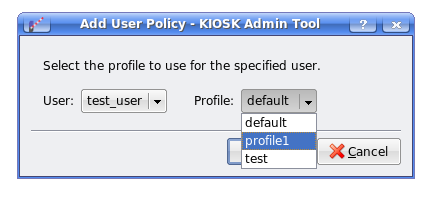
\includegraphics[width=8.5cm]{obrazky/KioskToolKDE3/prirazeni_profilu_uzivateli.png}
    \caption{Dialogy pro přiřazení profilů}
    \label{fig:kt3_prirazeni}
\end{figure}
Při pohledu na obrazovku a dialogy pro přiřazení Kiosk profilů skupinám
a uživatelům je nutné si připomenout, že když má uživatel přířazen svůj vlastní
profil, nevztahují se na něj profily pro skupiny kterých je členem. To program
nijak nezvýrazňuje. Bylo by dobré, kdyby poskytoval nějaký pohled, který by
ukazoval všechny profily efektivní pro uživatele.

\begin{figure}[h]
    \centering
    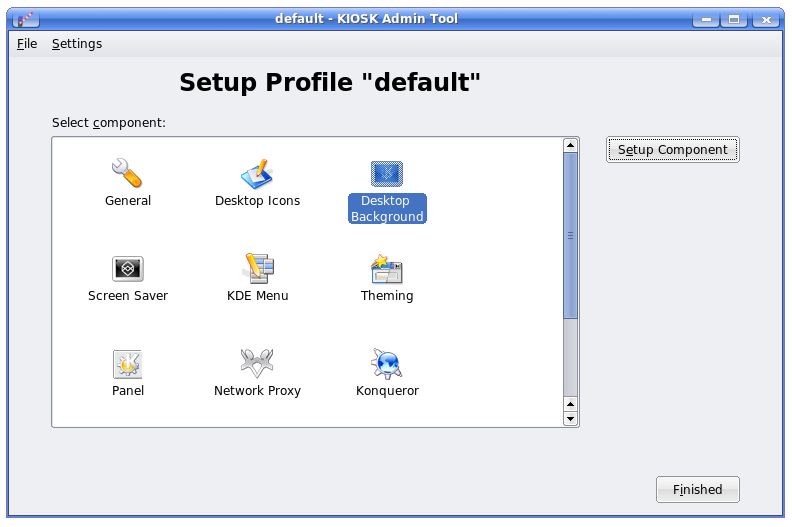
\includegraphics[width=8.5cm]{obrazky/KioskToolKDE3/seznam_komponent.png}
    \caption{Dialog s nastavením profilu}
    \label{fig:kt3_nast_prof}
\end{figure}
Dialog pru úpravu profilu \ref{fig:kt3_nast_prof} je mohem zajímavější. Je možné
z něj spouštět KCM moduly a části systému KDE a tak docílit toho, že KioskTool
může využít již existující funkcionalitu. Není proto nutné znovu 'vymýšlet kolo'
a uživatel pro nastavení Kiosk profilů používá stejné nástroje jako pro normální
nastavení. Tato původní verze nástroje KioskTool definuje všechny moduly
a jejich vlastnosti v jednom velkém XML souboru.

\begin{figure}[h]
    \centering
    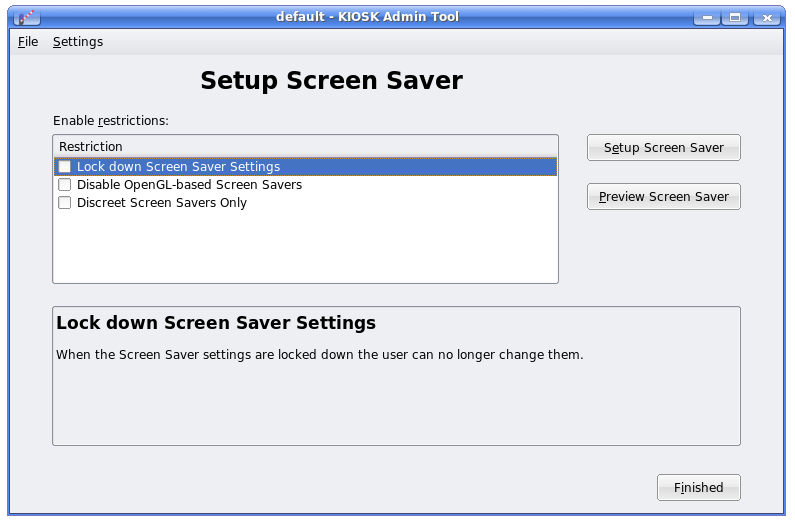
\includegraphics[width=8.5cm]{obrazky/KioskToolKDE3/ukazka_komponenty.png}
    \caption{Dialog jedné komponenty nástroje}
    \label{fig:kt3_nast_komp}
\end{figure}
Na obrázku \ref{fig:kt3_nast_komp} je vidět jak taková komponenta vypadá
v akci. Uživatel může uzamčít obrázek na pozadí plochy a ukázat si náhled tohoto
obrázku (náhled ve smyslu, že se pozadí plochy dočasně zamění). Zde by asi bylo
lepší místo náhledu otvírat KCM modul pro nastavení plochy a případně nějaký
režim pro rozvržení plasmoidů  na ní. Zejména kvůli tomu, že v KDE4 je původně %!REF! plasma
jednoduchá plocha nahrazena plochou plasma a tam je mnohem více věcí
k nastavování.

I při krátké době nutné na seznámení s nástrojem (KioskTool 1.0 v Kubuntu 9.04)
jsem narazil na fatální chyby, kdy se bez zjevného důvodu zhroutil. Nebude tedy
možné se spolehnout na korektnost kódu.

\begin{figure}[h]
    \centering
    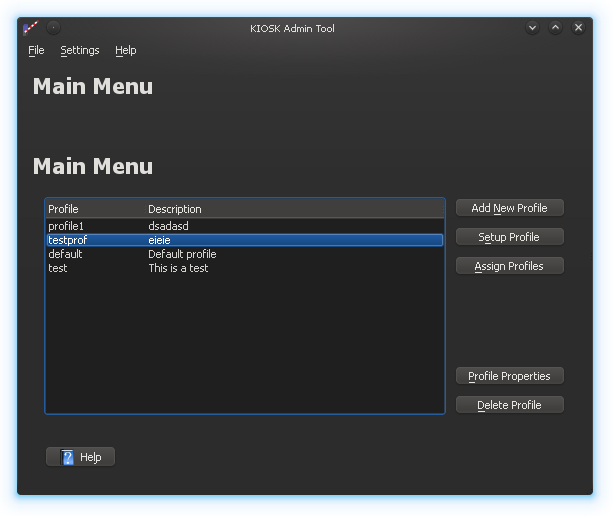
\includegraphics[width=8.5cm]{obrazky/KioskToolKDE4/kiosktool_kde4.png}
    \caption{=U}
    \label{fig:kt4_uvod}
\end{figure}

Port nástroje do KDE4 \ref{fig:kt4_uvod} již existuje, i když je značně
nedokončený.  %Ref: Kdo portoval, kde lze najít, proč toho nechal tak brzo?
Původní nastavení pomocí velkého XML souboru bylo odstraněno a nahrazeno mnoha
menšími .ini soubory. To má za účel umožnit ostatím autorům napsat pro jejich
aplikace moduly do nástroje KioskTool. Nástroj ztratil většinu svých modulů,
schopnost spouštět KCM moduly a náhledy, své pěkné (i když zbytečné) obrázkové
vzezření a získal několik dalších chyb. Zdá se ale, že na něm stále někdo
pracuje. %ref: Luboš Luňák?

\section{PolicyKit}
\begin{figure}[h]
    \centering
    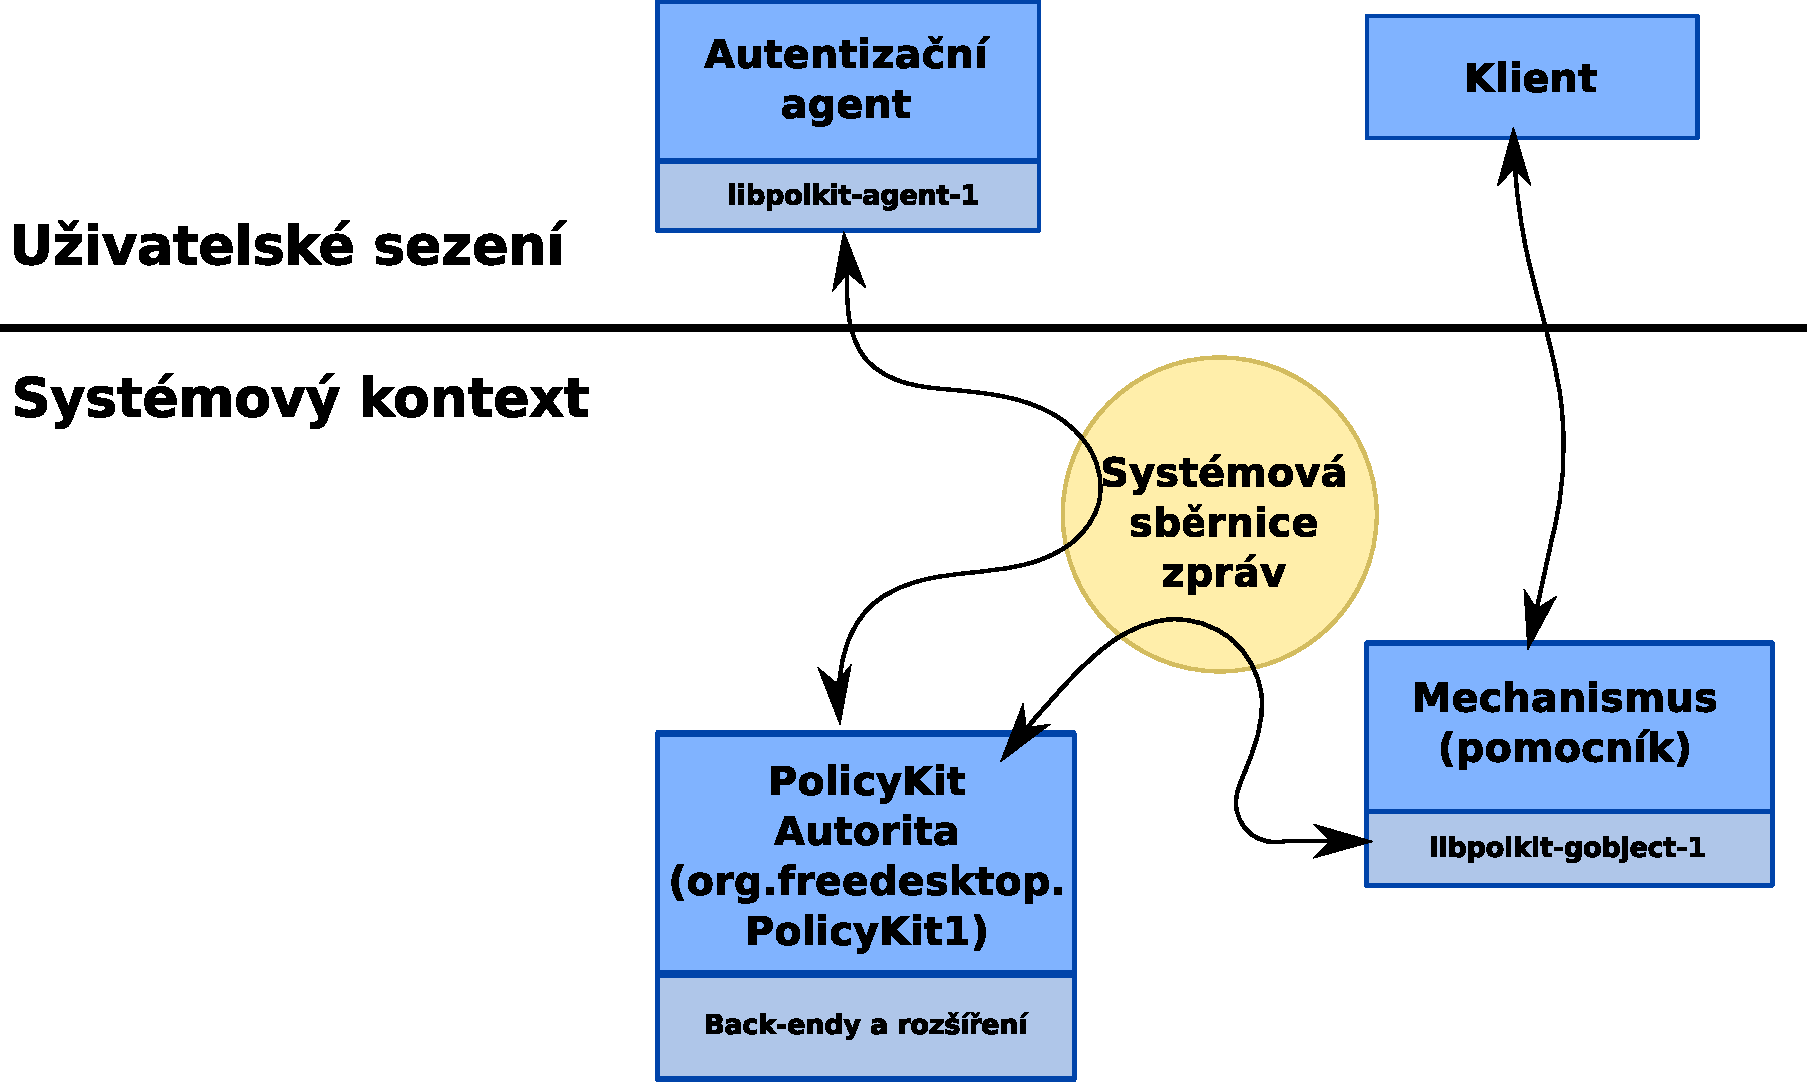
\includegraphics[width=8.5cm]{obrazky/polkit-architecture-vector-cz.pdf}
    \caption{Architektura systému PolicyKit}
    \label{fig:polkit_arch}
\end{figure}
PolicyKit (nebo také polkit), je systém umožňující autentizovat uživatele
a autorizovat akce, které tito uživatelé provádějí. Je to systém velmi modulární
a přenechává implementaci mnohých svých funkcí zásuvným modulům a programům,
které jej využívají.

Mezi nejzákladnější části tohoto systému patří démon polkitd (PolicyKit
Authority), který se stará o uložení databáze možných akcí a povolení. Další
částí, implementovanou prostředími jako je Gnome nebo KDE je tzv. autentizační
agent. To je program, který například uživateli zobrazí okno pro zadání hesla,
pokud je potřeba ověřit jeho totožnost. Pro ověření se používá pomocný program
s nastaveným setuid bitem.% REF!
Třetí komponentou je 'mechanismus' nebo 'pomocník' - zde se jedná o službu pro
vykonání privilegovaných akcí místo uživatele. Čtvrtou a poslední komponentou
je Klient - program, který využívá služeb systému PolicyKit. Jednotlivé
komponenty spolu komunikují pomocí IPC mechanismu DBUS.% REF IPC, REF DBUS!

Nad PolicyKitem je postavena knihovna polkit-qt. Poskytuje v zásadě stejné
funkce jako PolicyKit a lépe je integruje do prostředí knihoven QT. % REF!

Polkit-kde je nadstavbou nad knihovnou polkit-qt, která implementuje autentizačí
agent pro prostředí KDE a KCM modul pro úpravu akcí povolených pro uživatele
a skupiny.

Zatím jediným způsobem uložení povolených akcí v PolicyKitu je tzv. lokální
autorita. Je to výchozí implementace PolicyKit autority a využívá lokálně
uložených textových souborů s příponou .pkla. Efektivní seznam povolených akcí
se získá služením těchto souborů. Je tedy možné mít například jeden soubor
s výchozím nastavením instalovaný z distribučního balíčku a druhý s lokálním
nastavením, vytvořený administrátorem.

\begin{figure}[h]
    \centering
    \begin{verbatim}
                   /var/lib/polkit-1
                   └── localauthority
                       ├── 10-vendor.d
                       │   └── 10-desktop-policy.pkla
                       ├── 20-org.d
                       ├── 30-site.d
                       ├── 50-local.d
                       ├── 55-org.my.company.d
                       │   └── 10-org.my.company.product.pkla
                       └── 90-mandatory.d

                   /etc/polkit-1
                   └── localauthority
                       ├── 10-vendor.d
                       │   └── 01-some-changes-from-a-subvendor.pkla
                       ├── 20-org.d
                       ├── 30-site.d
                       ├── 50-local.d
                       ├── 55-org.my.company.d
                       │   └── 10-org.my.company.product.pkla
                       └── 90-mandatory.d
    \end{verbatim}
    \caption{Struktura složek pro PolicyKit Local Authority s několika .pkla soubory}
    \label{fig:pkit_la}
\end{figure}

Local Authority pro ně zavádí poměrně propracovanou strukturu \ref{fig:pkit_la}.
Pořadí načítání je určeno řazením složek a souborů v nich podle názvu. Pokud je
stejně pojmenovaný soubor v obou umístěních (ve /var/lib/ i /etc/), nejdříve se
zpracuje ten ve /var/.
%REF: cite man stránka pklocalauthority
Ve struktuře \ref{fig:pkit_la} by pořadí vypadalo takto:
\begin{itemize}
\item 10-desktop-policy.pkla
\item 01-some-changes-from-a-subvendor.pkla
\item 10-org.my.company.product.pkla (z /var)
\item 10-org.my.company.product.pkla (z /etc)
\end{itemize}

\section{KAuth}
KAuth je nové rozhraní pro autorizaci v KDE. Je postaveno na již existujících 
rozhraních v operačních systémech. V OS na bázi Linuxu je to zpravidla
PolicyKit, v OSX pak framework Authorization Services. Podporu pro nová
rozhraní je možné přidat pomocí zásuvných modulů.

Pomocí KAuthu je možné autorizovat akce uživatele. Zásuvný modul se stará
o veškeré ověřování akcí. Z pohledu PolicyKitu je zde aplikace používající
KAuth v roli klienta.
Další funkce poskytovaná KAuthem je vytvořit pokud možno co nejjednodušší
program, který pak bude v odpověď na autorizovanou akci spuštěn příslušným
autorizačním rozhraním. Takovýto program se nazývá KAuth pomocník (helper).
Pomocník a aplikace která ho využívá mohou do jisté míry komunikovat oběma směry
a je také možné sledovat průběh dlouho trvající akce uvnitř pomocníka. KAuth
pomocník je rozšířením PolicyKit pomocníka o tyto zjednodušené komunikační
funkce.

Převedení KAuth providel (soubory .actions) a KAuth pomocníků do formy
srozumitelné pro jednotlivé zásuvné moduly se provádí během kompilace a KAuth
nepodporuje provádění změn v nich po kompilaci. Také neumožňuje měnit
autorizované uživatele a skupiny pro akce - to je přenecháno KControl modulu
pro nastavení PolicyKitu obsaženému v balíku polkit-kde. Další nepodporovanou
částí je jakákoliv idea bezpečnostních profilů přiřazovaných uživatelům
a skupinám. Nic takového není ani v PolicyKitu.

\subsection{PolicyKit KControl modul (KCM)}
\chapter{Změny v~KAuthorized, KAuth}
\section{Slepá ulička: statický .actions soubor a integrace KAuth do KAuthorized}
\section{Slepá ulička: KConfig uvnitř KAuth pomocníka}
\section{Řešení}
\chapter{Úpravy nátroje KioskTool}
\section{Uživatelské rozhraní}
\section{Integrace KAuth}
\section{Spouštění KCM modulů}
\chapter{Další možný postup a návrh systematických změn v KDE}
\chapter{Testování a začlenění do KDE}
\chapter{Závěr}
\cite{fitWeb}
%=========================================================================
